\documentclass[8pt, landscape, a4paper]{extarticle}

% --- 核心宏包 ---
\usepackage[UTF8]{ctex}
\usepackage[margin=0.8cm, top=1cm, bottom=1.3cm]{geometry}
\usepackage{multicol}
\usepackage{xcolor}
\usepackage{tcolorbox}
\usepackage{enumitem}
\usepackage{amsmath}
\usepackage{amssymb}
\usepackage{fontspec}
\usepackage{tikz}
\usetikzlibrary{arrows.meta, shapes}

% --- 去掉页码 ---
\pagestyle{empty}

% --- 颜色定义 (Teal 主题) ---
\definecolor{headerblue}{RGB}{0, 150, 136}     % Teal
\definecolor{navcolor}{RGB}{211, 84, 0}        % 导航橙
\definecolor{intuitioncolor}{RGB}{41, 128, 185}% 直觉蓝
\definecolor{accentcolor}{RGB}{192, 57, 43}    % 强调红
\definecolor{section2}{RGB}{142, 68, 173}      % 紫色
\definecolor{dividergray}{RGB}{220, 220, 220}

% --- 全局设置 ---
\setlength{\parindent}{0pt}
\setlength{\columnsep}{0.4cm} 
\linespread{1.1} 

% --- 列表样式 ---
\setlist[itemize]{leftmargin=1.2em, nosep, itemsep=2pt, topsep=2pt, label=$\textcolor{headerblue}{\vcenter{\hbox{\tiny$\bullet$}}}$ }
\setlist[description]{leftmargin=0.2em, style=sameline, nosep, itemsep=2pt, font=\bfseries}

% --- Box 样式 ---
\newtcolorbox{mybox}[2][]{%
  colback=white,
  colframe=#2,
  coltitle=white,
  boxrule=1pt,             
  arc=2mm,                 
  left=4pt, right=4pt, top=3pt, bottom=3pt, 
  toptitle=3pt, bottomtitle=3pt, 
  fonttitle=\bfseries\sffamily\large,
  title={#1},
  after skip=5pt          
}

% --- 自定义命令 ---
\newcommand{\subt}[1]{{\vspace{2pt}\textbf{\large \textcolor{black}{#1}}}}

\newcommand{\boxdesc}[1]{%
    \textit{\small \textcolor{gray}{#1}}%
    \par\vspace{2pt}%
    {\color{dividergray}\hrule height 0.5pt}%
    \vspace{2pt}%
}

\newcommand{\sepline}{%
    \par \vspace{3pt}%
    {\color{dividergray}\hrule height 0.5pt}%
    \par \vspace{3pt}%
}

% 公式间距
\setlength{\abovedisplayskip}{3pt}
\setlength{\belowdisplayskip}{3pt}

\begin{document}

% --- 页眉 ---
\begin{center}
    {\Huge \textbf{\sffamily \textcolor{headerblue}{信息论 Information Theory Cheat Sheet}}} \\
    \vspace{0.2cm}
    {\large \texttt{The Physics of Data: From Entropy to Channel Capacity}}
\end{center}

% --- 开始四栏布局 ---
\begin{multicols*}{4}

% === 第一栏 ===

\begin{mybox}[️ 场景导航 (Use Cases)]{navcolor}
    \boxdesc{遇到什么问题 $\to$ 用什么工具}
    \begin{itemize}[itemsep=2pt]
        \item \textbf{数据压缩} $\to$ 熵 / 霍夫曼编码
        \item \textbf{模型评估} $\to$ 交叉熵 / KL 散度
        \item \textbf{特征选择} $\to$ 互信息 (Mutual Info)
        \item \textbf{通信带宽} $\to$ 信道容量 (Shannon Limit)
        \item \textbf{加密强度} $\to$ 完美保密性
        \item \textbf{决策树分裂} $\to$ 信息增益 (Information Gain)
    \end{itemize}
\end{mybox}

\begin{mybox}[1. 熵与不确定性 (Entropy)]{headerblue}
    \boxdesc{信息的度量单位}
    
    \subt{香农熵 (Shannon Entropy)}
    衡量分布 $P$ 的混乱程度 (平均惊奇度)。
    $$ H(X) = - \sum_{x} p(x) \log_2 p(x) $$
    \begin{itemize}
        \item \textbf{单位}: Bit (底数为2), Nat (底数为e)。
        \item \textbf{性质}: $H(X) \ge 0$。均匀分布时最大。
    \end{itemize}
    \sepline
    
    \subt{联合熵与条件熵}
    \begin{itemize}
        \item \textbf{联合熵}: $H(X,Y) = -\sum \sum p(x,y) \log p(x,y)$
        \item \textbf{条件熵}: $H(Y|X) = \sum p(x) H(Y|X=x)$
        \item \textbf{链式法则}: $H(X,Y) = H(X) + H(Y|X)$
    \end{itemize}
\end{mybox}

\begin{mybox}[2. 距离与相关性 (Measures)]{headerblue}
    \boxdesc{分布之间的“距离”}
    
    \subt{KL 散度 (Relative Entropy)}
    用分布 $Q$ 拟合真实分布 $P$ 时的\textbf{信息损失}。
    $$ D_{KL}(P||Q) = \sum p(x) \log \frac{p(x)}{q(x)} $$
    \begin{itemize}
        \item \textbf{非负}: $D_{KL} \ge 0$ (Gibbs 不等式)。
        \item \textbf{非对称}: $D_{KL}(P||Q) \neq D_{KL}(Q||P)$。
        \item \textbf{ML应用}: 最小化 KL $\iff$ 最大化似然。
    \end{itemize}
    \sepline
    
    \subt{互信息 (Mutual Information)}
    $X$ 和 $Y$ 共享的信息量。
    $$ I(X;Y) = H(X) - H(X|Y) = H(Y) - H(Y|X) $$
    \textit{直觉: 知道 $X$ 后,$Y$ 的不确定性减少了多少。}
\end{mybox}

\columnbreak

% === 第二栏 ===

\begin{mybox}[3. 信源编码 (Source Coding)]{headerblue}
    \boxdesc{如何压得更小 (无损压缩)}
    
    \subt{香农第一定理}
    最优码长 $L$ 的下界是熵 $H(X)$。
    $$ L \ge H(X) $$
    \sepline
    
    \subt{霍夫曼编码 (Huffman)}
    \begin{itemize}
        \item \textbf{策略}: 概率大的用短码,概率小的用长码。
        \item \textbf{算法}: 自底向上构建二叉树 (贪心)。
        \item \textbf{最优性}: 前缀码中最优。
    \end{itemize}
    \sepline
    
    \subt{算术编码 (Arithmetic)}
    将整个消息映射为 $[0, 1)$ 区间内的一个小数。
    \textit{优势: 突破整数位限制,逼近熵极限。}
\end{mybox}

\begin{mybox}[4. 信道编码 (Channel Coding)]{headerblue}
    \boxdesc{如何在噪声中传输 (纠错)}
    
    \subt{香农第二定理}
    只要传输速率 $R < C$ (信道容量),就存在一种编码能实现\textbf{任意低}的误码率。
    \sepline
    
    \subt{信道容量 (Capacity)}
    $$ C = \max_{p(x)} I(X;Y) $$
    \textbf{AWGN 信道公式}:
    $$ C = B \log_2 (1 + \text{SNR}) $$
    ($B$: 带宽, SNR: 信噪比)。
    \textit{启示: 增加带宽或信噪比都能提升网速。}
\end{mybox}

\columnbreak

% === 第三栏 ===

\begin{mybox}[5. 连续熵 (Differential)]{headerblue}
    \boxdesc{连续变量的世界}
    
    \subt{微分熵}
    $$ h(X) = - \int f(x) \log f(x) dx $$
    \begin{itemize}
        \item \textbf{注意}: 可以是负数!(不再代表比特数)。
        \item \textbf{最大熵}: 给定方差 $\sigma^2$,\textbf{高斯分布}熵最大。
    \end{itemize}
    \sepline
    
    \subt{AEP (渐进均分性)}
    大数定律的信息论版本。
    绝大多数序列都是“典型序列”,其概率 $\approx 2^{-nH(X)}$。
\end{mybox}

\begin{mybox}[6. 机器学习视角 (ML View)]{headerblue}
    \boxdesc{AI 的损失函数之源}
    
    \subt{交叉熵 (Cross Entropy)}
    $$ H(P, Q) = H(P) + D_{KL}(P||Q) $$
    $$ = -\sum p(x) \log q(x) $$
    \begin{itemize}
        \item \textbf{分类任务}: 真实标签 $P$ 是 One-hot,预测 $Q$ 是 Softmax。
        \item 最小化交叉熵 $\iff$ 最小化 KL 散度。
    \end{itemize}
    \sepline
    
    \subt{最大熵原理 (MaxEnt)}
    在满足约束的条件下,选择熵最大的分布 (最无偏见的假设)。
    \textit{例子: 没有任何信息时,假设为均匀分布。}
\end{mybox}

\begin{mybox}[7. Python / Scipy 实战]{headerblue}
    \boxdesc{代码工具箱}
    \begin{itemize}
        \item \texttt{from scipy.stats import entropy}
        \item \textbf{熵}: \texttt{entropy(pk, base=2)}
        \item \textbf{KL散度}: \texttt{entropy(pk, qk)}
        \item \textbf{互信息}: \texttt{sklearn.metrics.mutual\_info\_score}
    \end{itemize}
\end{mybox}

\columnbreak

% === 第四栏 ===

\begin{mybox}[8. 高阶概念 (Advanced)]{headerblue}
    \boxdesc{前沿探索}
    
    \subt{信息瓶颈 (Information Bottleneck)}
    深度学习理论:层与层之间应尽可能压缩输入信息 $I(X;T)$,同时保留输出信息 $I(T;Y)$。
    \sepline
    
    \subt{科尔莫哥洛夫复杂度 (K-Complexity)}
    描述一个对象所需的\textbf{最短程序}长度。
    \textit{不可计算,是熵的算法版本。}
    \sepline
    
    \subt{费雪信息 (Fisher Information)}
    观测数据 $X$ 包含参数 $\theta$ 的信息量。
    $$ I(\theta) = E[(\frac{\partial}{\partial \theta} \log f(X;\theta))^2] $$
    \textit{Cramer-Rao 下界: 方差 $\ge 1/I(\theta)$。}
\end{mybox}

\vspace*{\fill}

\begin{mybox}[ 核心直觉 (Intuition)]{intuitioncolor}
    \boxdesc{“比特是宇宙的原子。”}
    
    % TikZ 矢量图: 韦恩图展示 H(X), H(Y), H(X|Y), I(X;Y)
    \begin{center}
    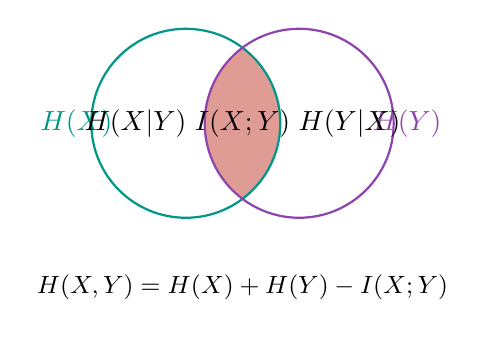
\begin{tikzpicture}[scale=0.8]
        % 定义圆
        \def\firstcircle{(0,0) circle (1.5cm)}
        \def\secondcircle{(1.8,0) circle (1.5cm)}

        % 填充 I(X;Y)
        \begin{scope}
            \clip \firstcircle;
            \fill[accentcolor!50] \secondcircle;
        \end{scope}
        
        % 轮廓
        \draw[thick, headerblue] \firstcircle node[left=0.8cm] {$H(X)$};
        \draw[thick, section2] \secondcircle node[right=0.8cm] {$H(Y)$};
        
        % 标注
        \node at (0.9,0) {$I(X;Y)$};
        \node at (-0.8,0) {$H(X|Y)$};
        \node at (2.6,0) {$H(Y|X)$};
        
        % 解释文字
        \node[below=1.8cm] at (0.9,0) {\small $H(X,Y) = H(X) + H(Y) - I(X;Y)$};
    \end{tikzpicture}
    \end{center}

    \hspace{1em}信息论告诉我们,\textbf{信息}是可以被精确度量的物理量,就像质量和能量一样。
    \vspace{4pt}
    
    \subt{三大核心视角}
    \begin{itemize}[itemsep=4pt]
        \item \textbf{惊奇度 (Surprise)}: 
        太阳从东边升起不包含信息 (概率=1, 熵=0)。太阳没升起才包含巨大信息。概率越小,信息量越大。
        
        \item \textbf{相关性即共享}: 
        互信息 $I(X;Y)$ 是比“相关系数”更本质的指标。它衡量了两个变量共享了多少比特。如果 $X$ 和 $Y$ 独立,互信息为 0。
        
        \item \textbf{编码即理解}: 
        如果你能把数据压缩得很小,说明你理解了它的规律 (模型好)。压缩率是智能的度量。
    \end{itemize}
    
    \vspace{6pt}
    \centering\textit{\footnotesize 宇宙由原子组成,但其本质是比特。}
\end{mybox}

\end{multicols*}

\end{document}
